\section{Likelihood inference}

Given a sequence of samples \( \mathbf X = ( X^{(1)}, \dots, X^{(N)} ) \) and model \( \mathcal{M}_{\theta \in \Theta} \), \( \Theta \subset \mathbb{R}^d \) maximize the log-likelihood function \(   \mathrm{argmax}_{\theta \in \Theta} \; \ell_{\mathbf X}(\theta) \), where \( \ell_{\mathbf X}(\theta) = \log\left( \prod^N_{i=1} f_\theta(X^{(i)}) \right) \). The \textbf{score equations} are 
\begin{align*}
  \begin{cases}
    \frac{\partial \ell_\mathbf X}{\partial\theta_1}(\theta) = 0 \\
    \frac{\partial \ell_\mathbf X}{\partial\theta_2}(\theta) = 0 \\
\vdots \\
\frac{\partial \ell_\mathbf X}{\partial\theta_d}(\theta) = 0 \\
  \end{cases}
\end{align*}
\textbf{Question:} What is the algebraic structure of the score equations?

\subsection{Maximum likelihood degree}

Assume a discrete model \( \mathcal{M}_\Theta \subset \Delta_{r - 1} \) with state space \( [r] \). The log-likelihood function is 
\begin{align*}
  \ell_{\mathbf X}(\theta) = \sum^r_{j=1} u_j \log(p_j(\theta)).
\end{align*}
Observe that if the \( p_j \)s are rational functions, then so are the score equations 
\begin{align*}
  \frac{\partial \ell_{\mathbf X}}{\partial\theta_k}(\theta) = \sum^r_{j=1}  \frac{u_j}{p_j} \frac{\partial p_j}{\partial\theta_k}(\theta) = 0.
\end{align*}

\begin{defi}[Maximum likelihood degree]
  The number of complex solutions (if finite) to the score equations for generic \( u \) is called the \textbf{maximum likelihood degree} of the parametric discrete model.
\end{defi}

The ML degree is an algebraic measure of \emph{complexity}. The best case if the ML degree is one, then there is a unique solution.

We need to check that the ML degree is well-defined.

\begin{prop}[ML degree is well-defined]
  For generic data \( u \in \mathbb N^r  \), the number of complex solutions is independent of \( u \).
\end{prop}

\begin{proof}
  Consider the coefficient field \( \mathbb C(\mathbf u) \). Assume \( p_j(\theta) = \frac{f_j}{g_j}(\theta) \) for all \( j= 1, \dots, r \). The log likelihood function becomes \( \sum^r_{j=1}u_j \cdot (\log(f_j(\theta)) - \log(g_j(\theta))) \). The score functions are \( \sum_{j=1}^r u_j (\frac{1}{f_j} \frac{\partial f_j}{\partial \theta_k}(\theta) - \frac{1}{g_j} \frac{\partial g_j}{\partial \theta_k}(\theta)) = 0 \) for all \( k=1, \dots, d \). Multiply by \( \prod_{j=1}^r f_j g_j \) and we define an ideal 
  \begin{align*}
    I = \left( \prod_{j=1}^r f_jg_j \sum_{j=1}^r u_j \left(\frac{1}{f_j} \frac{\partial f_j}{\partial \theta_k}(\theta) - \frac{1}{g_j} \frac{\partial g_j}{\partial \theta_k}(\theta)\right) : k = 1, \dots, d \right).
  \end{align*}
  Define \( J = I : \left(\prod_{j=1}^r f_jg_j\right)^\infty \) and compute \( V(J) \). The ML degree is the number of complex solutions \( \theta \) in \( V(J) \).
\end{proof}

\begin{eg}[What does generic mean?]
  Suppose we have the following score equation for some model
  \begin{align*}
    u_1 \theta^2 + u_2 \theta  + u_3 = 0.
  \end{align*}
  Here, generic \( u = (u_1,u_2,u_3) \) means that \( u_1 \neq 0 \) and \( u_2^2 - 4u_1u_3 \neq 0 \).
\end{eg}

\begin{eg}[Twisted cube]
Suppose have the following model 
\begin{align*}
  \mathcal{M}_{\theta \in [0,1]} = \left\{ \frac{1}{1 + \theta + \theta^2 + \theta^3} \begin{bmatrix} 1 \\ \theta \\ \theta^2 \\ \theta^3 \end{bmatrix} : \theta \in [0,1] \right\} \subset \Delta_3.
\end{align*}
Note that this is the log-linear model for the twisted cube with 
\begin{align*}
  \mathbf A = \begin{bmatrix}
    1 & 1& 1 &1 \\
    0 & 1 & 2 & 3 
  \end{bmatrix}, \quad p_1 \mapsto \theta_1, \quad p_2 \mapsto \theta_1 \theta_2, \quad p_3 \mapsto \theta_1 \theta_2^2, \quad p_4 \mapsto \theta_1 \theta_2^3.
\end{align*}
Define \( s = \frac{1}{1 + \theta + \theta^2 + \theta^3} \). The likelihood function is 
\begin{align*}
  L_{u}(\theta) = s^{u_0} (s\theta)^{u_1}(s\theta^2)^{u_2}(s\theta^3)^{u_3} = s^{u_0 + u_1 + u_2 + u_3} \theta^{u_1 + 2u_2 + 3u_3}.
\end{align*}
The log-likelihood function is
\begin{align*}
  \ell_u(\theta) = u_+ \log(s) + (u_1 + 2u_2 + 3u_3) \log(\theta).
\end{align*}
Calculating the score equations
\begin{align*}
  3(u_+ - u_3)\theta^3 + 2(u_+ - u_2)\theta^2 + (u_+ - u_1)\theta - (u_1 + u_2^2 + u_3^3) = 0,
\end{align*}
we get that the ML degree is three.
\end{eg}

\begin{eg}[Binomial random variable]
  Let \( X \) be a binomial random variable with two trials. We have the parametrization 
  \begin{align*}
    \theta \mapsto \begin{bmatrix}
      (1 - \theta)^2 \\
      2\theta(1 - \theta) \\
      \theta^2
    \end{bmatrix} \in \Delta_2.
  \end{align*} 
  The log-likelihood function is 
  \begin{align*}
    \ell_{u}(\theta) &= 2u_0 \log(1 - \theta) + u_1 \log(2\theta(1- \theta)) + 2u_2 \log(\theta) \\
    &= u_1 \log(2) + (u_1 + 2u_2)\log(\theta) + (2u_0 + u_1)\log(1 - \theta).
  \end{align*}
  Take the derivative, and we see that the ML degree is one.
\end{eg}

\begin{eg}[Independence model]
  Let \( X \indep Y \), so the joint distribution is parametrized by 
  \begin{align*}
    p_{ij} = \theta_i \theta_j.
  \end{align*}
  Let's say \( \mathcal{X} = \mathcal{Y} = [2] \). Then 
  \begin{align*}
    (\theta_1, \theta_2) \mapsto \begin{bmatrix}
      \theta_1 \theta_2 & \theta_1 (1 - \theta_2) \\
      (1 - \theta_1) \theta_2 & (1 - \theta_1)(1 - \theta_2)
    \end{bmatrix} = \mathbf p.
  \end{align*}
  The log-likelihood function \(  \ell_u(\theta_1, \theta_2)  \) is 
  \begin{gather*}
   u_{11}\log(\theta_1 \theta_2) + u_{12}\log(\theta_1(1 - \theta_2)) + u_{21} \log((1-\theta_1)\theta_2) + u_{22}\log((1 - \theta_1)(1 - \theta_2)) \\ 
   = \log(\theta_1)(u_{11} + u_{12}) + \log(\theta_2)(u_{11} + u_{21}) + \log(1 - \theta_1)(u_{21} + u_{22})\\ + \log(1 - \theta_2)(u_{12} + u_{22}).
  \end{gather*}
  Compute the score equations 
  \begin{align*}
    \frac{\partial}{\partial\theta_1}\ell_u(\theta_1, \theta_2) = \frac{u_{11} + u_{12}}{\theta_1} - \frac{u_{21} + u_{22}}{1-\theta_1} = 0 \\
    \frac{\partial}{\partial\theta_2}\ell_u(\theta_1, \theta_2) = \frac{u_{11} + u_{21}}{\theta_2} - \frac{u_{12} + u_{22}}{1-\theta_2} = 0 \\
  \end{align*}
  Then 
  \begin{align*}
    (1 - \theta_1)(u_{11} + u_{12}) = \theta_1(u_{21} + u_{22}) \\
    (1 - \theta_2)(u_{11} + u_{21}) = \theta_2(u_{12} + u_{22}),
  \end{align*}
  and 
  \begin{align*}
    \theta_1 = \frac{u_{11} + u_{12}}{u_{++}} \quad \text{ and } \quad \theta_2 = \frac{u_{11} + u_{21}}{u_{++}}.
  \end{align*}
\end{eg}

\subsection*{Multivariate normal model}

We see in this section that in case of multivariate normal random vectors, the score equations are rational in \( \theta = (\mu, \Sigma) \in \mathbb{R}^m \times \mathrm{PD}_m \). The log-likelihood function is (see Proposition \ref{mle:multivariate-normal}) 
\begin{align*}
  \ell_{X}( \mu, \Sigma) &= 
  -\frac{N}{2}   (m\log(2\pi) +  \log(\mathrm{det}(\Sigma))) -\frac{1}{2}\sum_{i=1}^N (X^{(i)} - \mu)^T \Sigma^{-1} (X^{(i)} - \mu) \\
  &= -\frac{N}{2}\left( m \log(2\pi) + \log\det(\Sigma) + \mathrm{tr}(\Sigma^{-1}S) + (\bar X - \mu)^T \Sigma^{-1}(\bar X - \mu) \right).
\end{align*}
We write 
\begin{align*}
  \sum_{i=1}^N (X^{(i)} - \mu)^T \Sigma^{-1} (X^{(i)} - \mu) 
  &= \sum_{i=1}^N (X^{(i)} - \bar X + \bar X - \mu)^T \Sigma^{-1} (X^{(i)} - \bar X + \bar X - \mu)\\
  &= \sum_{i=1}^N (X^{(i)} - \bar X)^T\Sigma^{-1}(X^{(i)} - \bar X) + (\bar X - \mu)^T \Sigma^{-1} (\bar X - \mu) \\
  &= N \mathrm{tr}(S \Sigma^{-1}) + \sum_{i=1}^N(\bar X - \mu)^T \Sigma^{-1} (\bar X - \mu) \\
  &= N \left(\mathrm{tr}(S \Sigma^{-1}) + (\bar X - \mu)^T \Sigma^{-1} (\bar X - \mu)\right).
\end{align*}
So, the log-likelihood function can be expressed in terms of the sufficient statistic \( T(X) = (\bar X, S) \):
\begin{align*}
  \ell_{X}( \mu, \Sigma) &= 
  -\frac{N}{2}   (m\log(2\pi) +  \log(\mathrm{det}(\Sigma))) -\frac{N}{2}\mathrm{tr}(S \Sigma^{-1}) - \frac{N}{2} (\bar X - \mu)^T \Sigma^{-1} (\bar X - \mu).
\end{align*}
\begin{mdframed}
\begin{cor}[Full gaussian model]
  The score equations of the full Gaussian model \( \Theta = \mathbb{R}^m \times \mathrm{PD}_m \) are rational in \( \mu \) and \( \Sigma \); unique solutions are 
\begin{align*}
  \hat \mu = \bar X \quad \text{and} \quad \hat \Sigma = S;
\end{align*}
hence the ML degree is one.
\end{cor}
\end{mdframed}


MLE reduces to a simpler problem if we fix \( \Sigma = \mathrm{ID}_m \) and only estimate \( \mu \) from some parameter space \( \Theta_1 \subset \mathbb R^m \).

\begin{mdframed}
\begin{prop}[Restricted mean and identitiy covariance matrix]
Let \( X \in \mathbb R^m \) be a normal random vector. Assume we want to estimate the parameter of the model \( \mathcal{M}_{\theta \in \Theta} \) for \( \Theta = \Theta_1 \times \left\{ \mathrm{ID}_m \right\} \) and \( \Theta \subset \mathbb R^m \). Then the maximum likelihood is equivalent to the least squares method.
\end{prop}
\end{mdframed}

\begin{proof}
  We need to estimate \( \mu \in \Theta_1 \); using maximum likelihood, we have
  \begin{align*}
    \hat \mu = \mathrm{argmax}_{\mu \in \Theta_1} (\bar X - \mu)^T (\bar X - \mu) =  \mathrm{argmax}_{\mu \in \Theta_1} \lVert \bar X - \mu \rVert^2.
  \end{align*}
  This means we search for the \( \mu \) in \( \Theta_1 \) that is closest to the sample mean.
\end{proof}

We define the \textbf{ED degree} (Euclidean distance degree) to be the number of critical points of the Euclidean distance \( \lVert \bar X - \mu \rVert^2 \) function for generic \( \bar X \). Critical points are the solutions to the score equations \( \frac{\partial}{\partial \mu} \lVert \bar X - \mu \rVert^2 = 0 \). 

\begin{figure}[H]
  \centering
  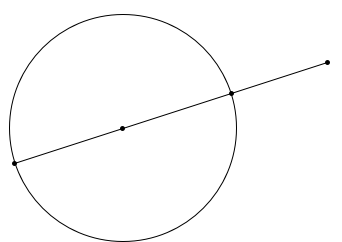
\includegraphics[width=0.4\textwidth]{assets/eddegree-circle.png}
  \caption{The ED degree of a line is one, of a circle two, of a parabola three and of an ellipsoid four.}
\end{figure}

\begin{cor}[ML Degree equals ED degree]
  The ML degree equals the ED degree for Gaussian models with unit covariance.
\end{cor}

\begin{cor}[Rationality of score equations for Gaussian models with unit covariance]
  The score equations for Gaussian models with identity covariance matrix are rational in \( \mu \).
\end{cor}

\begin{eg}[Nodal cubic]
  Assume \( \Theta_1 = \left\{ \begin{bmatrix}t^2 - 1\\ t(t^2 - 1)\end{bmatrix} \mid t \in \mathbb{R} \right\} \); this is a nodal cubic.
  \begin{figure}[H]
    \centering
    \includegraphics*[width=0.5\textwidth]{assets/nodal-cubic.jpg}
  \end{figure}
  Assume the covariance is fixed to be the identity matrix. Then the ML degree equals the ED degree; find \( \mu \in \mathbb{R}^2 \) in \( \Theta_1 \) such that it minimizes
  \begin{align*}
    \lVert \bar X - \mu \rVert^2 = (\bar X_1 - t^2 + 1)^2 + (\bar X_2 - t(t^2 - 1))^2.
  \end{align*}
  Computing the derivative yields 
  \begin{align*}
    &\frac{\partial}{\partial t} \left((\bar X_1 - t^2 + 1)^2 + (\bar X_2 - t(t^2 - 1))^2\right) \\&= 2(\bar X_1 - t^2 + 1) \cdot (-2t) + 2(\bar X_2 - t(t^2 - 1)) \cdot (-3t^2 + 1).
  \end{align*}
  Setting this to zero, we get a polynomial score equation in \( t \) of degree \( 5 \). The ED degree equals 5.
\end{eg}

\begin{mdframed}
\begin{prop}[Unrestricted mean and restricted covariance matrix]
  Let \( \Theta = \mathbb R^m \times \Theta_1 \), where \( \Theta_1 \subset \mathrm{PD}_m \). Then the maximum likelihood estimate is
  \begin{align*}
    \hat \mu = \bar X \quad \text{and} \quad \hat \Sigma = \mathrm{argmin}_{\Sigma \in \Theta_1} \log\det(\Sigma) + \mathrm{tr}(\Sigma^{-1}S).
  \end{align*}
  Alternatively, in terms of the precision matrix \( K = \Sigma^{-1} \), we have
  \begin{align*}
    \hat \mu = \bar X \quad \text{and} \quad \hat K = \mathrm{argmax}_{K \in \Theta_1^{-1}} \log\det(K) - \mathrm{tr}(KS).
  \end{align*}
\end{prop}
\end{mdframed}

\begin{prop}[Centered model and restricted covariance matrix]
  Another special case is given if we have a centered model, that is \( \Theta = \left\{ 0 \right\} \times \Theta_1 \). Then we have the same result as in the previous proposition but now with \( S = \frac{1}{N} \sum^N_{i=1}x^{(i)}{x^{(i)}}^T \).
\end{prop}

\begin{eg}[Full independence and centered model]
  Let \( \mathbf X = (X_1, X_2, X_3) \) be a random normal vector.
  Assume \( \Theta \) is centered and given by full independence \( X_1 \indep (X_2, X_3), X_2 \indep (X_1,X_3) \) and \( X_3 \indep (X_1,X_2) \). Then 
  \begin{align*}
    \Theta_1 = \left\{ \begin{bmatrix}
        \sigma_{11} & 0 & 0 \\
        0 & \sigma_{22} & 0 \\
        0 & 0 & \sigma_{33}
    \end{bmatrix}\right\} \subset \mathrm{PD}_3 \quad \text{and} \quad \Theta_1^{-1} = \left\{ 
    \begin{bmatrix}
      \frac{1}{\sigma_{11}} & 0 & 0 \\
      0 & \frac{1}{\sigma_{22}} & 0 \\
      0 & 0 & \frac{1}{\sigma_{33}}
    \end{bmatrix}
     \right\}  \subset \mathrm{PD}_3.
  \end{align*}
  Further, assume that we are given the sample covariance matrix
  \begin{align*}
    S = \begin{bmatrix}
      s_{11} & s_{12} & s_{13} \\
      s_{21} & s_{22} & s_{23} \\
      s_{31} & s_{32} & s_{33}
    \end{bmatrix}.
  \end{align*}
  Let \( a = \sigma_{11}^{-1} \), \( b = \sigma_{22}^{-1} \) and \( c = \sigma_{33}^{-1} \).
  The likelihood function if \( K \) is
  \begin{align*}
    \log \det K - \mathrm{tr}(KS) = \log(abc) - (s_{11}a + s_{22}b + s_{33}c ).
  \end{align*}
  Take the derivative with respect to \( a \), \( b \) and \( c \) and set to zero. We get that the ML degree is one and 
  \begin{align*}
    \hat \Sigma = \begin{bmatrix}
      s_{11} & 0 & 0 \\
      0 & s_{22} & 0 \\
      0 & 0 & s_{33}
    \end{bmatrix}.
  \end{align*}
\end{eg}

\begin{eg}[Bivariate centered model and restricted covariance matrix]
  Let \( \mathbf X =(X_1, X_2) \) be a random normal vector. Assume it is centered and 
  \begin{align*}
    \Theta_1 = \left\{ \begin{bmatrix}1 & \rho \\ \rho & 1\end{bmatrix} \mid \rho \in (-1,1) \right\}.
  \end{align*}
  The parameter \( \rho \) is the correlation between \( X_1 \) and \( X_2 \), i.e. \( \rho = \mathrm{Corr}(X_1, X_2) \). Assume we have sample covariance matrix 
  \begin{align*}
    S = \begin{bmatrix}
      s_{11} & s_{12} \\ s_{12} & s_{22}
    \end{bmatrix};
  \end{align*}
  note that this matrix is symmetric. Also, we compute the precision matrix 
  \begin{align*}
    \Sigma^{-1} = K = \frac{1}{1 - \rho^2} \begin{bmatrix}
      1 & - \rho \\ -\rho & 1
    \end{bmatrix}
  \end{align*}
  The log-likelihood is 
  \begin{align*}
    \ell_{\mathbf X}(\theta) \propto \log \det \Sigma + \mathrm{tr}(\Sigma^{-1}S) = \log(1 - \rho^2) + \frac{1}{1 - \rho^2} (s_{11} + s_{22} -2 \rho s_{12}).
  \end{align*}
  Take the derivative with respect to \( \rho \) and setting this to zero gives
  \begin{align*}
    \frac{\partial}{\partial\rho}  \ell_{\mathbf X}(\theta) \propto \frac{-2\rho}{ 1 - \rho^2} + \frac{-2s_{12}(1 - \rho^2) - (s_{11} + s_{22} - 2\rho s_{12}) \cdot (-2 \rho)}{(1 - \rho^2)^2} = 0.
  \end{align*}
  The score equation is 
  \begin{align*}
    \rho^3 - s_{12}\rho^2 + (s_{11} + s_{22} - 1)\rho - s_{12} = 0.
  \end{align*}
  The ML degree is three.
\end{eg}

\begin{eg}[Ungeneric data]
  Continuing the last example, suppose we have ``ungeneric'' data \( S \) with \( s_{12} = 0 \). Then, the score equation becomes
  \begin{align*}
    \rho(\rho^2 + s_{11} + s_{22} - 1)= 0.
  \end{align*}
  One MLE solution is \( \hat \rho = 0 \). If \( s_{11} + s_{22} > 1 \), then \( \hat \rho = 0 \) is the unique solution, and we have \( \hat \Sigma = \begin{bmatrix}
    1 & 0 \\ 0 & 1
  \end{bmatrix} \). For the other case \( s_{11} + s_{22} < 1 \), we get two further solutions on top of \( \hat \rho = 0 \); this is the generic case.
\end{eg}

\begin{eg}
  Assume a centered normal model and \( \Theta_1 = \left\{ \Sigma \in \mathrm{PD}_4 \mid \sigma_{12} = \sigma_{34} = 0 \right\} \); this means that \( X_1 \indep X_2 \) and \( X_3 \indep X_4 \). We have
  \begin{align*}
    \Sigma = \begin{bmatrix}
      \sigma_{11} & 0 & \sigma_{13} & \sigma_{14} \\
      0 & \sigma_{22} & \sigma_{23} & \sigma_{24} \\
      \sigma_{13} & \sigma_{23} & \sigma_{33} & 0 \\
      \sigma_{14} & \sigma_{24} & 0 & \sigma_{44}
    \end{bmatrix}
  \end{align*}
  Assume we observed this random (and generic) sample covariance matrix 
  \begin{align*}
    S = \begin{bmatrix}
      19 & 3 & 5 & 7 \\
      3 & 23 & 11 & 13 \\
      5 & 11 & 31 & -1 \\
      7 & 13 & -1 & 37
    \end{bmatrix};
  \end{align*}
  note that this matrix is positive definite. We want to use Macaulay2 to compute the critical solutions of 
  \begin{align*}
    \log \det \Sigma + \mathrm{tr}(\Sigma^{-1}S).
  \end{align*}
  To compute \( \Sigma^{-1} \) we use \(     \Sigma^{-1} = \frac{1}{\det \Sigma}\mathrm{adj}(\Sigma)
  \).
  If we compute the critical solutions of \(  \log \det \Sigma + \mathrm{tr}(\Sigma^{-1}S) \) with Macaulay2, we need to first turn the equations into a polynomial. Define \( f = \det \Sigma \) and \( L = \mathrm{tr}(\mathrm{adj}(\Sigma) S) \). Then the log-likelihood becomes
  \begin{align*}
    \ell = \log f + \frac{1}{f}L.
  \end{align*}
  So the score equations are
  \begin{align*}
   \frac{1}{f}\frac{\partial f}{\partial \sigma_{ij}} + \frac{\frac{\partial L}{\sigma_{ij}}f - L \frac{\partial f}{\sigma_{ij}}}{f^2} = 0.
  \end{align*}
  Multiply by \( f^2 \), and we get an ideal in the polynomial ring. Compute the vanishing set of the saturated ideal with respect to \( (f) \); we need the saturation to remove unwanted zeroes that were introduced by \( f \). Then, we see that the ML degree is 17.
\end{eg}


\subsection{Discrete models with constraints}

Let \( \mathcal{M} \subset \Delta_{r - 1} \) be a family of discrete models.

\begin{defi}[Likelihood function in projective space]
  Let \( V \subset \mathbb P^{r - 1} \) be an irreducible projective variety over \( \mathbb{C} \), and let \( \mathbf u \in \mathbb{N}^r \) be a vector of counts. The likelihood function \( L_\mathbf u: V \to \mathbb{C} \) is defined as
  \begin{align*}
    L_\mathbf u (\mathbf p) = \frac{p_{1}^{u_1} \dots p_r^{u_r}}{(p_1 + \dots + p_r)^{u_1 + \dots + u_r}}.
  \end{align*}
  Note that if \( \mathbf p \in \Delta_{r - 1} \), we recover the usual likelihood function. Moreover, \( L_\mathbf u  \) is a rational function in \( \mathbf p \) of degree zero (the numerator is of degree \( u_+ \) and the denominator has also degree \( u_+ \)).
\end{defi}

Previously, we assigned the ML degree to statistical models; now we assign the ML degree to projective varieties.

\begin{defi}[ML degree of projective varieties]
  The ML degree of \( V \) is the number of critical points \( \mathbf{p} \) of \( L_\mathbf u \) for generic \( \mathbf u \) on \( \mathbf{p} \in V_{\text{reg}} \setminus \mathcal{H} \) where \( \mathcal{H} = V(p_1...p_r(p_1 + ... + p_r)) \). 
\end{defi}

Since \( \mathbf p \) is constrained, we use Lagrange multipliers to find the critical points of \( L_\mathbf u \).

\begin{remark}[Lagrange multipliers]
  Assume \( V = (f_1, \dots, f_k) \). These are our \( k \) constraints.
  We optimize the log of \( L_\mathbf u \) plus the Lagrange multipliers:
  \begin{align*}
    \mathcal{L}_\mathbf u(\mathbf p, \lambda) = \left(\sum_{i=1}^r u_i \log(p_i)\right) - u_+\log(p_+) + \sum^k_{j=1} \lambda_j f_j.
  \end{align*}
  So, the score equations are 
  \begin{align*}
    \frac{\partial \mathcal{L}_\mathbf u}{\partial p_i}(\mathbf p)  &= \frac{u_i}{p_i} - \frac{u_+}{p_+} + \sum_{j=1}^k \lambda_j \frac{\partial f_j}{\partial p_i}(\mathbf p) = 0 \\
    \frac{\partial \mathcal{L}_\mathbf u}{\partial \lambda_j}(\mathbf p) &= f_j(\mathbf p) = 0.
  \end{align*}
\end{remark}

\begin{eg}[Binomial model with two trials]
  Let \( X \) be a discrete random variable. Assume \( V \) is given by \( p_1^2 - 4p_0p_2 \). Given counts \( \mathbf u = (u_0, u_1, u_2) \) find \( \theta \) such that \(\mathbf p_\theta \in V \) that maximizes \( L_\mathbf u \). Note that the implicit equation characterizes the binomial model with two trials. So in the end, we should end up with the ML estimator for the binomial model. Let's see if this is indeed the case.
  
  The Lagrange function is
  \begin{align*}
    \mathcal{L}_\mathbf u (\mathbf p, \lambda) = u_0 \log(p_0) + u_1 \log(p_1) + u_2 \log(p_2) - \lambda p_1^2 +  \lambda 4p_0p_2.
  \end{align*}
  We have 
  \begin{align*}
    \frac{\partial}{\partial p_0}: \frac{u_0}{p_0} - \frac{u_+}{p_+} + 4\lambda p_2 = 0 \\
    \dots
  \end{align*}
  Solve for \( p_0,p_1,p_2 \) and \( \lambda \) in terms of \( u_0, u_1 \) and \( u_2 \) gives 
  \begin{align*}
    \begin{bmatrix}
      \hat p_0 \\ \hat p_1 \\ \hat p_2
    \end{bmatrix} =
    \begin{bmatrix}
      \frac{(2u_0 + u_1)^2}{4(u_0 + u_1 + u_2)^2} \\
      \frac{(2u_0 + u_1)(u_1 + 2u_2)}{2(u_0 +  u_1 + u_2)^2} \\
      \frac{(u_1 + 2u_2)^2}{4(u_0 + u_1 + u_2)^2}
    \end{bmatrix}
  \end{align*}
  This is consistent with \( \mathrm{Bin}(2, \theta) \) where 
  \begin{align*}
    \hat \theta = \frac{u_1 + 2u_2}{2(u_0 + u_1 + u_2)}.
  \end{align*}
  Note that if by chance the count \( \mathbf u \) lies in \( V(p_1^2 - 4p_0p_2) \) then \( \lambda = 0 \) and \( \hat{\mathbf p} = \frac{1}{\mathbf u_+}(u_0,u_1,u_2)\).
\end{eg}

\begin{eg}[Independence model]
  Assume the statistical model 
  \begin{align*}
    \mathcal{M} = \left\{ \begin{bmatrix} p_{11} & p_{12} \\ p_{21} & p_{22} \end{bmatrix} \in \Delta_3 \mid p_{11}p_{22} - p_{12}p_{21} = 0 \right\} 
  \end{align*}
  What is this model? What is the MLE? We know that this is the independence model \( X \indep Y \) for \( X,Y \in [2] \). The MLE is given by 
  \begin{align*}
    \hat p_{ij} = \frac{u_{i+}u_{+j}}{u_{++}^2}.
  \end{align*}
  If we had computed critical solutions to the Lagrange equation we would have obtained the exact same result as above.
\end{eg}

June Huh proved in 2014 that if the ML degree of a variety is one, then  \( \hat{\mathbf p} \) is always a rational function in \( \mathbf u \) of degree zero where numerator and denominator are products of linear form.

\begin{defi}[Algebraic torus]
  The \textbf{algebraic torus} is \( (\mathbb{C}^*)^r = (\mathbb{C} \setminus \left\{ 0 \right\})^r \).
\end{defi}

\begin{defi}[Very affine variety]
  A \textbf{very affine variety} is a set of the form \( V \cap (\mathbb{C}^*)^r \) where \( V \subset \mathbb{C}^r \) is a variety.
\end{defi}

Our statistical model live in the probability simplex; from an algebraic geometry point of view, we consider our model to live in a very affine variety.

\begin{thm}[June Huh, 2014]
  Let \( X \) be a discrete random variable with state space \( \mathcal{X} = [r] \), and \( V \) a very affine variety.
  Let \( \mathrm{MLdegree}(V) = 1 \). Then, there exists \( \mathbf h  \in \mathbb{C}^r \) and a matrix \( \mathbf B \in \mathbb{Z}^{n \times r} \) where all columns sum to zero such that 
  \begin{align*}
    \hat p_j(u_1, \dots, u_r) = h_j \prod^n_{i=1}\left( \sum^r_{k=1} b_{ik} u_k \right)^{b_{ij}}
  \end{align*}
  \( (\mathbf B,\mathbf h) \) is called a \textbf{Horn pair}.
\end{thm}

\begin{eg}[Binomial model with two trials]
  Let \( \mathbf h = \begin{bmatrix}
    1 & 2 & 1
  \end{bmatrix} \) and \( \mathbf B = \begin{bmatrix}
    2 & 1 & 0 \\ 0 & 1 & 2 \\ -2 & -2 & -2
  \end{bmatrix} \). Then 
  \begin{align*}
    \hat p_0 &= (2u_0 + 1u_1)^2  (0u_0 + u_1 + 2u_2)^0  (-2u_0 - 2u_1 - 2u_2)^{-2}\\ &= \frac{(2u_0 + u_1)^2}{(-2u_0 - 2u_1 - 2u_2)^{2}}
  \end{align*}
  Similarly, 
  \begin{align*}
    \hat p_1 &= 2\left( (2u_0 + u_1) (u_1 + 2u_2) (-2u_0 - 2u_1 - 2u_2)^{-2} \right) \\
    \hat p_2 &= (2u_0 + u_1)^0 (u_1 + 2u_2)^{2} (-2u_0-2u_1-2u_2)^{-2}
  \end{align*}
\end{eg}

\begin{eg}[Independence model]
  Assume \( X \indep Y \), \( X,Y \in [2] \). We know \( \hat p_{ij} = \frac{p_{i+}p_{+j}}{p_{++}^2} \). What is \( \mathbf h \) and \( \mathbf B \)? We have 
  \begin{align*}
    \hat p_{11} = \frac{(u_{11} + u_{12})(u_{11} + u_{21})}{u_{++}^2} \\
    \hat p_{12} = \frac{(u_{11} + u_{12})(u_{12} + u_{22})}{u_{++}^2} \\
    \hat p_{21} = \frac{(u_{21} + u_{22})(u_{11} + u_{21})}{u_{++}^2} \\
    \hat p_{22} = \frac{(u_{21} + u_{22})(u_{12} + u_{22})}{u_{++}^2}.
  \end{align*}
  Then 
  \begin{align*}
    \mathbf h = \begin{bmatrix}
      4 & 4 & 4 & 4
    \end{bmatrix} \quad \text{and} \quad \mathbf B = \begin{bmatrix}
      1 & 1 & 0 & 0 \\ 0 & 0 & 1 & 1 \\  1 & 0 & 1 & 0 \\ 0 & 1 & 0 & 1 \\ -2 & -2 & -2 & -2
    \end{bmatrix}.
  \end{align*}
  Note that \( \mathbf{B} \) contains \( \mathbf{A} \) as a submatrix, where \( \mathbf{A} \) is the matrix from the log-linear model. 
\end{eg}

\begin{thm}[June Huh, Euler characteristic]
  Let \( V \subset (\mathbb{C}^*)^r \) be a very affine variety of dimension \( d \). If \( V \) is smooth (i.e. it contains no singular points), then \( \mathrm{MLdegree}(V) = (-1)^d \mathcal{X}(V) \), where \( \mathcal{X}(V) \) is the Euler characteristic of \( V \).
\end{thm}

\subsection{Log-affine linear models}
We now consider the MLE of log-affine linear models.

\begin{mdframed}  
\begin{thm}[Birch's Theorem]
  Let \( \mathcal{M} \)  be a \emph{discrete} regular exponential family.
  Let \( A \in \mathbb{Z}^{k \times r} \) such that \( \mathbf{1} \in \mathrm{rowspan}(A) \), \( \mathbf h \in \mathbb{R}^r_{> 0} \) and \( \mathbf{u} \) vector of counts from \( N \) i.i.d. samples. Then the MLE, if it exists, is the unique solution to the equation 
  \begin{align*}
    A \mathbf{\bar u} = A \mathbf p
  \end{align*}
  with \( \bar{\mathbf u} = \frac{1}{N}\mathbf u \) is the empirical distribution and \( \mathbf p \in \mathcal{M}_{A,h} \). Note that if we do not restrict \( \mathbf p \) to lie in the probability simplex, then there may exist multiple solutions;.
\end{thm}
\end{mdframed}

\begin{proof}
  This follows from Corollary \ref{mle-discrete-regular-exp}, which concerned regular, not necessarily discrete, exponential families. Note that \( \mathbf u \) is always a sufficient statistic for a discrete model. \( A \mathbf u \) is the minimal sufficient statistic for a log-linear model.

  Let \( \mathbf X = (X^{(1)}, \dots, X^{(N)}) \) be an i.i.d. sample with state space \( \mathcal{X} = [r]^{N} \). Then, 
  \begin{align*}
    T(\mathbf X) = \sum_{i=1}^N T(X^{(i)}).
  \end{align*}
  Recall that for log-affine linear models, the columns \( \mathbf a_{\cdot j} \) of \( A \) consists of \( T(1), \dots , T(r) \). So, we get
  \begin{align*}
    T(\mathbf X) =  \sum^r_{i=1} u_i T(j) = \sum^r_{i=1} u_i \mathbf a_{\cdot i} = A \mathbf u.
  \end{align*}
  Next, note that 
  \begin{align*}
    \mathbb{E}[T(X)] = N \cdot \mathbb{E}[T(X^{(N)})] = N \sum^r_{i=1} p_i T(i) = N A \mathbf p.
  \end{align*}
  Hence, \(     N A \mathbf p = \mathbb{E}[T(X)] = T(X) = A \mathbf u
  \).
\end{proof}

Let \( A = \begin{bmatrix}
 \vline & \dots & \vline \\
 \mathbf a_{\cdot 1} & \dots & \mathbf a_{\cdot r} \\
  \vline & \dots & \vline
\end{bmatrix} \in \mathbb{Z}^{k \times r} \) such that \( \mathbf{1} \in \mathrm{rowspan}(A) \). Let \( \mathbf h \in \mathbb{R}^r_{> 0} \). We can define a lattice polytope by \( P(A) = \mathrm{conv}\left\{ a_1, \dots, a_r \right\} \subset \mathbb{R}^k \). A point \( p \) lies in the relative interior of a polytope \( P = \mathrm{conv}\left\{ p_i \right\} \) if there exists a positive convex combination of the vertices that equals \( p \); note that not every convex combination for \( p \) need be positive.

\begin{mdframed}
\begin{thm}[Existence of MLE]
  Let \( \mathcal{M}_{A, \mathbf h} \) be a discrete exponential family. The MLE exists for \( \mathcal{M}_{A, \mathbf{h}} \) if and only if \( A \bar{\mathbf u}  \in \mathrm{relint}(P(A))\).
\end{thm}
\end{mdframed}

\begin{proof}
  \( \implies \):
  Assume the MLE exists for \( \mathcal{M}_{A, \mathbf h} \). By Birch's Theorem there exists a \( \mathbf p \in \mathcal{M}_{A, \mathbf h} \) such that \( A \mathbf p = A \mathbf{\bar u} \). Recall that \(\mathbf  p \in \mathcal{M}_{A, \mathbf{h}} \) means that \( \mathbf p \) lies in the interior of the probability simplex. Hence, \( A \mathbf{\bar u} \) lies in the relative interior of \( P(A) \) since all \( p_i > 0 \) for \( i = 1, \dots, r \).

  If \( \mathbf b = A \mathbf{\bar u} \in \mathrm{relint}(A) \), then there exists positive \( \mathbf v \in \mathbb{R}^r_{> 0} \) such that \( N\mathbf b = A \mathbf{v} \). Observe that the likelihood \( \prod p_i^{u_i} \) can be replaced by \( \prod p_i^{v_i} \) since \( A \mathbf u = A \mathbf{v} \). Next, note that on the boundary of \( \mathbf{p} \in \mathcal{M}_{A, \mathbf{h}} \), the likelihood is zero because all exponents \( v_i > 0 \) and some \( p_i =0 \). Note that in the interior of \( \mathcal{M}_{A, \mathbf{h}} \) the likelihood is positive. Since the likelihood function of an exponential family is concave, a maximum is attained in the interior of \( \mathcal{M}_{A, \mathbf{h}} \).
\end{proof}

There are only two cases: if \( \bar{\mathbf u} \) lies on the boundary of \( P(A) \), then the MLE does not exist. If \( \bar{\mathbf u} \) lies in the relative interior of \( P(A) \), then the MLE exists and is unique.

\begin{cor}
  If all the components of \( \mathbf u \) are positive, then the MLE exists and is unique.
\end{cor}

\begin{eg}[Independence model]
  Consider \( \mathcal{M}_{X \indep Y} \) with \( X,Y \in [2] \). Does the MLE exist? For which data does it exist?
   
  \( \mathcal{M}_{X \indep Y} \) is a log-linear model with 
  \begin{align*}
    A = \begin{bmatrix}
      \vline & \vline & \vline & \vline \\
      \mathbf a_{\cdot 1} &  \mathbf a_{\cdot 2} &  \mathbf a_{\cdot 3} &  \mathbf a_{\cdot 4} \\
      \vline & \vline & \vline & \vline 
    \end{bmatrix} = \begin{bmatrix}
      1 & 1 & 0 & 0 \\
      0 & 0 & 1 &1 \\
      1 & 0 & 1 & 0 \\
      0 & 1 & 0 & 1 
    \end{bmatrix}.
  \end{align*}

  The polytope \( P(A) \subset \mathbb{R}^4 \) lives in \( \mathbb{R}^2 \). Assume we are given some data \( \mathbf u  \in \mathbb{N}^4\). If all \( u_i > 0 \), then the MLE exists. If some \( u_i =0 \), then it can go wrong.

  \begin{itemize}
    \item Let \( \mathbf u = (2,0,0,3) \). Then 
    \begin{align*}
      A \bar{\mathbf{u}} = \frac{1}{5}(2 \cdot \mathbf{a}_{\cdot 1} + 3 \cdot \mathbf{a}_{\cdot 4}) = \frac{1}{5}\begin{bmatrix}
        2 \\ 3 \\ 2 \\ 3
      \end{bmatrix}
    \end{align*}
    The point \( \frac{1}{5}\begin{bmatrix}
      2 & 3 & 2 & 3
    \end{bmatrix}^T \) lives in the relative interior of \( P(A) \) since we can find a positive convex combination of vertices of \( A \) such that 
    \begin{align*}
      \frac{1}{5}\begin{bmatrix}
        2 \\ 3 \\ 2 \\ 3
      \end{bmatrix} = A \begin{bmatrix}
        1 \\ 1 \\ 1 \\ 2
      \end{bmatrix}.
    \end{align*}

    \item Let \( \mathbf{u} = (1,0,1,0) \). Then \( A\bar{\mathbf{u}} = \frac{1}{2}(1,1,2,0) \). This lives on the boundary of the polyope; hence no MLE exists.
  \end{itemize}
\end{eg}

\subsection{Gaussian linear concentration models}

Let \( L \subset \mathbb{R}^{\frac{m(m+1)}{2}} \) be a linear space of matrices such that \( L \cap \mathrm{PD}_m \neq \emptyset \).
Recall the Gaussian linear concentration model \( \mathcal{M}_L \); this model consists of all normal distributions in \( \mathcal{N}(\cdot, \Sigma) \)  parametrized by \( \Sigma \in L^{-1} = \left\{ \Sigma \in \mathrm{PD}_m \mid \Sigma^{-1} \in L \right\} \). The likelihood is given by 
\begin{align*}
  \ell_K(S) = \log \det K - \mathrm{tr}(KS).
\end{align*}
A minimal sufficient statistic is \( T(X) = \pi_L(S) \), the orthogonal projection of the sample covariance matrix \( S \) onto the linear space \( L \).

\begin{thm}[MLE estimator for Gaussian linear concentration models]
  Let \( \Theta = \mathbb{R}^m \times L^{-1} \) be the parameter space of \( \mathcal{M}_L \). Let \( X^{(1)}, \dots, X^{(N)} \in \mathbb{R}^m \) i.i.d. sample. Then the MLE for \( (\mu, \Sigma) \in \Theta \), if it exists, is \( (\bar X, \hat \Sigma) \) where \( \hat \Sigma \) is the unique solution to 
  \begin{align*}
    \pi_L(\hat \Sigma) = \pi_L(S), \quad \hat \Sigma \in L^{-1}.
  \end{align*}
\end{thm}

\begin{prop}[Existence of MLE for Gaussian linear concentration models]
  The MLE exists for Gaussian linear concentration models if and only if \( \pi^{-1}_L(S) \neq \emptyset   \) if and only if \( \pi_L(S) \in \mathrm{relint(\mathcal{C}_L)} \); here \( \mathcal{C}_L \) denotes the cone of matrices in \( L \).
\end{prop}

\begin{eg}[Gaussian graphical models]
  The linear space \( L \) can be given by a Gaussian graphical model \( G \). It consists of matrices  
  \begin{align*}
    L = \left\{ (k_{ij})_{i,j}  \mid k_{ij} = 0 \iff \text{there is no edge between \( i \) and \( j \) in \( G \)}  \right\}.
  \end{align*}
  For instance, consider the following Gaussian graphical model 
  \begin{figure}[H]
    \centering
    % https://tikzcd.yichuanshen.de/#N4Igdg9gJgpgziAXAbVABwnAlgFyxMJZABgBpiBdUkANwEMAbAVxiRAEYQBfU9TXfIRTtyVWoxZsATN14gM2PASJl2Y+s1aIQAZll9FgoiLXUNk7QBZuYmFADm8IqABmAJwgBbJGRA4ISCIgABYwdFBskGCsPK4e3ohB-kg61KHhkQQxcu5eSFLUyYipIWER2lHZcXmIvkUFpRkVWTZcQA
\begin{tikzcd}
  1 \arrow[r, no head] \arrow[d, no head] & 2 \arrow[d, no head] \\
  3 \arrow[r, no head]                    & 4                   
  \end{tikzcd}
  \end{figure}
  There is no edge between \( (2,3)  \)  and \( (1,4) \); so \( L \) consists of matrices 
  \begin{align*}
    L = \left\{ \begin{bmatrix}* & * & * & 0 \\ * & * & 0 & * \\ * & 0 & * & * \\ 0 & * & * & *\end{bmatrix} \right\}.
  \end{align*}
\end{eg}

\begin{thm}[MLE for Gaussian graphical models]
  Let \( G \) be an undirected graph. The MLE estimator \( (\hat \mu, \hat \Sigma) \) of the Gaussian graphical model \( \mathcal{M}_G \) given sufficient statistic \( T(X) = (\bar X, S) \) is 
  \begin{align*}
    \bar \mu = \bar X \quad \text{and} \quad \hat \Sigma_{ij} = s_{ij}\; \text{if \( i \leftrightarrow j \in G \) or \( i=j \)}, \quad  \hat \Sigma^{-1}_{ij} =0 \; \text{if \( i \leftrightarrow j \notin G \)}
  \end{align*}
  provided the MLE exists. In words, whenever there is an edge between \( i \) and \( j \) in \( G \), we set \( \hat \Sigma_{ij} = s_{ij} \); when there is no edge, the \( (i,j) \)-th component of \( \hat \Sigma \) is only implicitly given by the inverse.
\end{thm}

\begin{eg}
  Consider the following Gaussian graphical model \( G \):
  \begin{figure}[H]
    \centering 
    % https://tikzcd.yichuanshen.de/#N4Igdg9gJgpgziAXAbVABwnAlgFyxMJZABgBpiBdUkANwEMAbAVxiRAEYQBfU9TXfIRTtS7KrUYs2AZm68QGbHgJEATOXH1mrRCFXdxMKAHN4RUADMAThAC2SESBwQk6kAAsYdKG0hhWPJY29oiOzkhkHl4+un4BFFxAA
\begin{tikzcd}
  1 &                                           & 2 \\
    & 3 \arrow[ru, no head] \arrow[lu, no head] &  
  \end{tikzcd}
  \end{figure}
  The linear space is 
  \begin{align*}
    L = \left\{ \begin{bmatrix}* & 0 & * \\ 0 & * & * \\ * & * & *\end{bmatrix} \right\}.
  \end{align*}
  What is \( \hat \Sigma \) of the graphical model \( \mathcal{M}_G \)? Assume we have data \( S \). Then, we know by the above theorem that 
  \begin{align*}
    \hat \Sigma = \begin{bmatrix}
      s_{11} &x & s_{13} \\
      x & s_{22} & s_{23} \\
      s_{13} & s_{23} & s_{33}
    \end{bmatrix}.
  \end{align*}
  The entry \( \hat \Sigma_{12} \) must be chosen in a way such that \( \hat \Sigma_{12}^{-1} = 0 \); using the formula \( \hat \Sigma^{-1}_{ij} = (-1)^{i+j} \frac{1}{\det \hat \Sigma} \mathrm{det}(\hat \Sigma_{ji}) \), we obtain 
  \begin{align*}
    \hat \Sigma^{-1}_{12} = (-1)^{1 + 2}\frac{1}{\det \hat \Sigma}(x s_{33} - s_{13}s_{23}) =0.
  \end{align*}
  So \( x =  \frac{s_{13}s_{23}}{s_{33}}\).
\end{eg}